\documentclass[12pt,a4paper,fleqn]{report}

\usepackage[utf8x]{inputenc}
\usepackage[T1]{fontenc}
\usepackage{lmodern}
\usepackage{amsmath}

\usepackage{graphicx} % Allows including images
\usepackage{caption}
\captionsetup[figure]{size=footnotesize}
\captionsetup{justification=centering}

\usepackage[section]{placeins}
\usepackage{float}

\usepackage{multirow}

\usepackage[toc]{appendix}
\usepackage{etoc}

\setlength{\mathindent}{5mm}

\usepackage{lipsum}
%\usepackage{showframe}

\renewcommand{\familydefault}{\sfdefault}

\title{%
	End-of-Studies Internship Report \\
	\large "Underwater Localisation for an Underwater Sensor Network" \\
}
\author{Antoine Maréchal}
\date{September 2017}

\begin{document}

\maketitle

\etocdepthtag.toc{mtchapter}
\etocsettagdepth{mtchapter}{subsection}
\etocsettagdepth{mtappendix}{none}
\setcounter{tocdepth}{1}
\tableofcontents

%\chapter*{Introduction}
%\addcontentsline{toc}{chapter}{Introduction}
%
%\lipsum[1-5]

\chapter{Context and objectives}

Underwater sensors have many application in various domains, such as oceanographic
data collection, pollution monitoring, offshore asset monitoring, disaster prevention, assisted navigation, and tactical surveillance applications.

Sub-sea monitoring is often realized by deploying underwater sensors to collect data for a limited period of time, then recover them. This has many disadvantage: impossibility of real-time monitoring, adaptation to changing conditions, or rectification of problems after deployment. As a result, there is a strong interest in developing network capable of both internal and external communications.

Due to the particularities of the underwater medium, the most viable technology for wireless underwater communications is the use of acoustic waves. This makes underwater networking highly challenging compared to terrestrial networks. A network of underwater intercommunicating devices is commonly called an \textbf{underwater acoustic sensor network}, or \textbf{UASN}.

\section{USMART project}

USMART aims to create a smart underwater sensing framework based on ultra-low-
cost wireless communication and sensing nodes (‘smart dust’). It is a collaboration between Heriot-Watt University (Edinburgh), Newcastle University, and University of York.

The key novel contributions of this project will be:
\begin{itemize}
	\itemsep0em
	\item Disruptive, low-cost technology enabling mass deployment with battery life of several years.
	\item Large scale underwater monitoring (>100 devices) with high spatio-temporal sampling rate.
	\item Rapid deployment and near real time data delivery (as opposed to data logging).
	\item Intelligent, adaptive sensing to maximise resource utilisation and fully exploit large scale.
\end{itemize}

The project is based on small, energy-efficient, performant underwater communication devices known as "nanomodems". This will be combined with energy efficient multiple access network protocols based knowledge of the underwater channel and intelligent, sparse sensing/localisation algorithms. A testbed near the Northumberland coast will serve to conduct real conditions trials.

This internship is part of the research on network localisation. Based on the known position of a few devices, acquired for example using GPS, the position of the other devices in the network must be determined using distributed algorithms.

\section{Terminology}

All devices that are part of an underwater network are called \textbf{nodes} of this network. In addition to the "nanomodems" described above, this may refer to devices such as surface buoys or unmanned underwater vehicles (UAVs).

A node whose position is not yet known is called \textbf{unlocalised}, while a node who has been able to estimate its own position is called \textbf{localised}. A group of nodes, or an entire network, can also be called localised if all the nodes in it are localised. The process of finding the position of a node, or several, is accordingly called \textbf{localisation}.

A localised node that serves as a point of reference to calculate the position of other node(s) is called an \textbf{anchor}. A node that can determine its position using external means instead of relying on anchors, and thus can serve as a starting point to the localisation process, is called an \textbf{initial anchor}. This may be, for example, a buoy equipped with a GPS receiver.

\chapter{Prior works}

\section{UASN typology}

There are many ways to categorize underwater sensor network. Some of them, such as the purpose of the network, have little relevance to the localisation problem. Others, such as the geometry of the network, are much more important. Q. Fengzhong et al., in their survey of localisation schemes \cite{survey} have proposed several criteria that are most relevant to the choice of localisation methods.

\subsection{Spatial coverage}

The network can be three-dimensional or two-dimensional (for examples, if all the nodes are lying on a flat seafloor). The same localisation methods can be used for both, with slight differences in implementations.

If the nodes are equipped by a depth sensor, the localisation problem can be reduced to two dimensions (by projecting all positions and distances in a horizontal plane), making the distinction irrelevant. No depth-aware version of the localisation methods have been implemented or tested.

\subsection{Node mobility}

If the position of the nodes change during the localisation process, then the localisation method needs to take into account and attempt to predict these movements. On the contrary, if they are stationary, then estimating their position is easier. This report considers networks that are stationary, at least over the time scale of the localisation process (several hours).

\subsection{Calculations assignment}

Localisations methods can be classified as \textbf{distributed} or \textbf{centralized}. One of our requirements is that the methods must be distributed: each node, based on communication with its neighbours, must calculate its own position and may or may not make it known to the rest of the network.

\subsection{Precision and measurements}

Some method only give a coarse estimate of the node's position, a region of space where it is located: they are usually based simply of which nodes are within range of each other, and are called "range-free". Methods called "range-based", on the other hand, rely on geometric measurements to calculate accurate estimations of the node's position. These are the methods we are interested in.

Among these methods, we can distinguish four categories, characterized by the measurements they use.
\begin{itemize}
	\itemsep0em
	\item Time of Arrival (\textbf{ToA}) methods use propagation times of messages to measure distances. The position of the node is found at the intersection of spheres centred on the anchors. However, this requires either time synchronization between the nodes (and thus expensive equipment), or back and forth communications (which are more costly in energy and time).
	\item Time Difference of Arrival (\textbf{TDoA}) methods only measures differences of distances; as a result, one-way communications are sufficient and synchronization between emitters and receivers are not necessary. The position of the node is found at the intersection of hyperboloids.
	\item Received Signal Strength Indicator (\textbf{RSSI}) measures distances, like ToA, but uses the attenuation of received signals to do so. Due to the characteristics of the underwater medium, this gives poor results, and as a consequence this method is seldom used in UASNs.
	\item Angle of Arrival (\textbf{AoA}) methods measure the direction from which signals are received to calculate positions. The position of the node is found at the intersection of planes, cones or lines. However, this is only possible with directional emitters or receivers (or both), which are more costly and bulky.
\end{itemize}
TDoA methods were considered the most promising, with (asynchronous) ToA a close second. AoA and RSSI methods were not considered, for the reasons given above.

\section{UPS and derivatives}

\subsection{Underwater Positioning Scheme}

The "Underwater Positioning Scheme" (UPS) is a small-scale, generic localisation method proposed by X. Cheng et al. \cite{ups}. It is based on time difference of arrival, which means that time synchronization is not needed, and only the anchors need to broadcast: the nodes to be localised are passive.

This method requires four anchors in order to obtain a unique solution, which cannot be coplanar. For example, three of them can be surface buoys (localised using GPS), and the fourth an underwater node (localised by an alternate methods, e.g. ToA, using the first three as anchors).

\begin{figure}[h]
	\centering
	\includegraphics[scale=0.35]{img/ups}
	\caption{%
	Example of anchor disposition in UPS
	}
\end{figure}

The anchors take turns broadcasting messages (called "beacons") in a predefined order: each anchor after the first waits for the beacon of its immediate predecessor before sending its own. This way, it is not possible for beacons to conflict (and thus be lost). Beacons contain information such as the coordinates of the anchor (if it hadn't been broadcast in advance), its position in the broadcasting order, and more importantly the delay between receiving the previous beacon and sending this one. For added precision, and to mitigate the possibility of transmission losses, the anchors can repeat their broadcasting cycle several times.

Knowing the speed of sound, the position of the anchors, the retransmission delays, and the relative time of arrival of the beacons, a node that has received all four beacons can calculate the distance difference between itself and the anchors, and from there its own position, using calculations detailed in appendix \ref{appendix:tdoa}. There is no theoretical limitation on the number of nodes that can be simultaneously located by this method. However, they all need to be within range of all four anchors.

The relative simplicity and energy efficiency (due to the small number of broadcasts) of this localisation method have made it fairly popular in the scientific literature, and several proposed schemes build upon it.

\subsection{Enhanced UPS}

H.P Tan et al. \cite{eups} have proposed several improvements on UPS, collectively called "Enhanced UPS" (E-UPS). The basic localisation principle is left untouched, but the changes make the scheme more resilient to various failure modes.

The article focuses on a situation where a single node (e.g. an underwater autonomous vehicle) is to be localised using an arbitrary (greater than four) number of point-of-reference nodes. Nevertheless, some of the ideas it introduces are potentially useful.

The first of these ideas is the dynamic determination of the anchors. Because UPS depends on a pre-determined set of anchors, the failure of any one of these nodes would mean the failure of the entire localisation process. E-UPS instead lets the node to be localised choose the four anchors among all reference nodes. The node initiate the localisation process by broadcasting a requested anchor set, and sends a termination message once it has been able to calculate its position.

The second idea is what the article call "time-out beaconing". Because of the sequential nature of UPS, it is especially vulnerable to transmission losses. If one anchor fails to receive the previous beacon, then the entire localisation sequence fails. In E-UPS, each anchor is given a time-out delay. If enough time passes after the initial request without receiving its predecessor's beacon, then the anchor will broadcast its beacon anyway. This ensures that the broadcasting sequence will complete no matter what, though it doesn't guarantee that all beacons will reach the nodes to be localised.

\subsection{Localisation Scheme for Large-Scale networks}

The "Localisation Scheme for Large-Scale networks" (LSLS) has been proposed by W. Cheng et al. \cite{lsls}. It is based on UPS and extends it to networks of any size. The article assumes depth projection is used: as a result, sets of three anchors (called golden, silver and bronze) are used, rather than four.

LSLS uses the same localisation process as UPS, but repeats it many times until the entire network is localised, using nodes localised in previous iterations as new anchors. The process begins with a set of initial anchors (e.g. surface buoys with GPS), which localise the nodes around them; then, a distributed process selects new anchor sets, which then localise more nodes, and so on until the entire network is localised.

New anchor sets are selected by the following process:

\begin{itemize}
	\itemsep0em
	\item All nodes that know their position are golden candidate, and set a timer (that depends on the distance to the anchors that localised them).
	\item If a candidate's timer runs out, then it becomes a golden anchor and broadcasts a notification to its neighbours.
	\item If a candidate receives one such broadcast before the end of the timer, then it registers this golden anchor, becomes a silver candidate, and sets a new timer (that depends on the distance to the golden anchor).
	\item The same process is repeated to select a silver anchor, then a bronze anchor.
\end{itemize}

Once the three anchors have been chosen, the golden anchor sends out the first beacon, followed by the silver and bronze anchors, according to the UPS method. The timers are calculated in such a way as to select anchor sets of appropriate sizes: smaller sets can locate new nodes in a larger area, resulting in a faster progress of the localisation process

This method can, in theory, eventually localise networks of any size, as long as they are dense enough to find new anchor sets. Since it is based on UPS, it shares its strong points: lack of synchronization requirement and overall simplicity of the localisation method proper. However, the amount of communications it entails is unclear, especially for the anchor selection process.

\chapter{Work performed}

\section{Simulation of UASNs}

In order to test the various localisation schemes found in the scientific literature, a way to simulate underwater sensor networks was needed. Several frameworks for such simulations exist already, such as NS-MIRACLE and its extension DESERT Underwater. However, since I was only looking to do proofs-of-concepts rather than in-depths simulations, the complexity of these solution would be a hindrance more than an asset.

Instead, I preferred to create a simple simulation environment for my own use. This simulator, developed in Python, offers basic features, but simplifies some aspects of the underwater medium and ignore others. These shortcomings are discussed below.

\subsection{Principles of the simulation}

A network of sensor is implemented as a collection of objects, each representing one node of the network, contained in a "simulation environment" object, which manages the communications between each of the nodes.

The simulation of the network over time is based on an event queue, which contain two kind of events:
\begin{itemize}
	\itemsep0em
	\item A periodical poll of the entire network (called a "tick" in the implementation), giving each node the opportunity to actualize its own status and possibly to broadcast a message.
	\item The reception of one such message by an individual node.
\end{itemize}

When a node decides to broadcast a message, the simulation environment determines which nodes are in range, and for each of them calculates the propagation time based on the distance between the sender and the recipient. Each of these time-stamped reception events are then added to the queue.

In the earliest versions, nodes could only broadcast on polling events. Later, the ability to reply directly after receiving a message was added. In this case, a slight delay is added to the propagation time, representing the computing time between reception and reply.

A secondary feature of the simulator object is the display of a 3D snapshot of the network, using the Python module $mpl\_toolkits.mplot3d$. How each node is displayed is defined in the node class. In general, a node is represented by a dot with a shape and color depending on its status (not localised, localised, anchor, etc). Other information about the node may be displayed as well, for example any position estimate it may have calculated, as well as the expected precision of the estimate. It is possible, as an option, to display snapshots of the simulation at set intervals of time while it runs.

Some parameters of the simulation are set when creating the simulator object (dimensions of the simulation space), others when it is run (duration of the simulation, logging options). Other parameters – polling period, broadcast range, speed of sound, for example – are defined in a separate file, along with other constants used by one or several node classes. This allows separate classes to easily share those parameters.

\subsection{Simulation of uncertainty}

In order to test the robustness of the methods tested, the simulation emulates the uncertainty inherent to real conditions in two ways: errors in propagation delays, and transmission failures.

The error in propagation delays consists simply in adding a Gaussian variation to the speed of sound. Tests were done with a mean value of 1500 m/s, and typical standard deviations of 1\% to 2\% (15 m/s to 30 m/s), up to 5\% (75 m/s) in some tests. These values are consistent with the speed of sound variations expected in real conditions.

Originally, these variations in the speed of sound were modelled as a noise: a new random variation was calculated for each transmission (emitter to receiver: each broadcast consists of as many transmissions as there are nodes in range). It quickly became apparent that this was a poor model, since in real conditions, the speed of sound varies continuously across space and time.

In later versions, the local speed of sound is interpolated from eight random values, one for each corner of the simulation space. These values are changed over the course of the simulation by small random increments. This more adequately models the continuity over time and space of the speed of sound. In order to make calculations easier, the propagation time is calculated using the speed of sound in the middle of the line between the emitter and the receiver, rather than integrating along it. Analysis shows that the difference is negligible.

Transmission failure are simulated with a simple transmission loss rate. When a node broadcasts a message, each node in range has a fixed chance to not receive it. Those random transmission failures are all independent and the probability does not depend on location or on past success or failures of the sender or the recipient. Because this feature was disabled in most of the later tests, it was never improved beyond this very basic model.

\subsection{Limitations}

The simulation does not model many of the intricacies of sound propagation in water: reflection against the seafloor or the surface, which result in duplicate messages being received, refraction through speed gradients, which can cause transmissions to take longer paths or be reflected entirely, to name a few. This affects both the calculation of propagation times, and more importantly the modelisation of transmission errors.

In particular, errors are treated as an all-or-nothing problem: either the message is received intact, or not at all. There is no simulation of corrupted or garbled messages, though this issue could be mitigated by employing error-detecting or -correcting codes, so the localisation algorithm wouldn't have to worry about it.

Likewise, communication range is simulated in an all-or-nothing fashion. Either a node is in range of the broadcast and it receives the message (chance of failure aside), or it is out of range and it does not receive anything. There is also no option to give nodes different transmission power or different receiver sensitivities: all transmissions have the same range.

The length of messages is also not considered, and as a consequence there is no limit on how many messages a node could receive in a given interval. In real conditions the bit-rate of underwater communication is rather low, and broadcasts might be several seconds long, depending on how much data they contain. If a node receive two overlapping messages, both could be rendered unintelligible. However, even though this problem is not present in the simulation, it is still possible to design localisation algorithms around it, and verify afterwards that no node received messages in close succession.

The desynchronized nature of the network is not simulated, either: when a node is polled, or receive a message, they are given the current time from the same simulated clock. This could easily be changed, by simply assigning to each node a random time shift at the beginning of the simulation. However, the absence of this feature does not prevent the simulation of algorithms that do not rely on synchronization, and for this reason it was not judged useful.

\section{UPS tests}

\subsection{Implementation}

The UPS tests were realized using three different types of nodes, each implemented in a different class.

The "master anchor" node is the first anchor in the broadcasting cycle. Only one such node is used at a time. It sends a pre-set number of beacons at regular intervals. The time between two broadcasts is chosen so that each cycle finishes before the next one begins. A higher number of cycles makes the process longer, but gives more resilience to transmission losses and greater accuracy.

The "anchor" nodes are the subsequent anchors in the broadcasting cycle. Three of these nodes are used at once. These nodes wait to receive the beacon from their predecessor, then broadcast a beacon of their own.

Beacons contain the following data:

\begin{tabular}{|l|l|p{9cm}|}
	\hline
	\textbf{value} & \textbf{type} & \textbf{explanation} \\
	\hline
	count	& int		&
	identifies the current broadcasting cycle \\
	\hline
	level	& int (0-3)	&
	position in the anchor order \\
	\hline
	x		& float		&
	horizontal coordinate of the node \\
	\hline
	y		& float		&
	horizontal coordinate of the node \\
	\hline
	z		& float		&
	vertical coordinate of the node \\
	\hline
	delay	& float		&
	duration between the sending of the level 0 beacon, and the transmission of this message \\
	\hline
\end{tabular}

\medskip

The latter is calculated by the anchor, by adding the delay data of the previous beacon, the propagation time of the beacon (itself calculated from the respective positions of the anchors), and the anchor's own retransmission delay.

The "sensor" nodes are the ones that must be located. Their role is passive: they listen to the beacons and register the data (time of arrival and delay). Then, after the anchors have finished broadcasting, they average this data and use it to calculate a position estimate. See appendix \ref{appendix:tdoa} for details on this calculation.

\subsection{Findings}

Testing demonstrates that UPS, if correctly used, is a reasonably accurate localisation method. This, in addition to its other qualities described above, make it a good starting point for large-scale localisation methods.

Simulations on networks around one kilometre in size, and with average speed of sound variation (30 m/s) find that position estimates are often within 10 meters of the actual positions.

Success and accuracy of UPS depends a lot on the disposition of the anchor set. An anchor set that is too "flat" (i.e. close to coplanar) is prone to greater localisation errors. Moreover, there are regions of space where localisation fails because there is no single solution to the equations, mostly around the anchors. For certain anchor dispositions, these regions may be excessively large.

The main disadvantage of UPS is, as noted before, its limited reach. The localisation methods tested thereafter keep the basic localisation principle, but seek to extend it iteratively to large-scale networks.

\begin{figure}[h]
	\centering
	\includegraphics[scale=0.4]{img/ups-test}
	\caption{%
	Result of a UPS simulation \\
	Black: master anchor and anchor nodes \\
	Blue: successfully localised sensor nodes \\
	Red: sensor nodes that could not be localised \\
	}
\end{figure}

\subsection{Error estimation}

One particular challenge of UPS is estimating the difference between the calculated position and the actual position of the node. This is especially important later on, when anchor sets must be chosen and accuracy of the node's position would be an important criteria. Unfortunately, no satisfactory solution to this problem was found.

Error estimation is only possible when several samples of TDoA data have been gathered, as a result of several broadcasting cycles by the anchors. The position estimate is a result of the average of this dataset, but its variance can be used to calculate an error estimate.

The first method attempted to estimate position and error was the following:
\begin{itemize}
	\itemsep0em
	\item From each sample, calculate a position
	\item Calculate the average of these points to obtain the position estimate
	\item Calculate the standard deviation of to obtain the error estimate
\end{itemize}
Since the samples are averaged after doing the localisation calculations, this method can be called "post-averaging".

\begin{figure}[h]
	\centering
	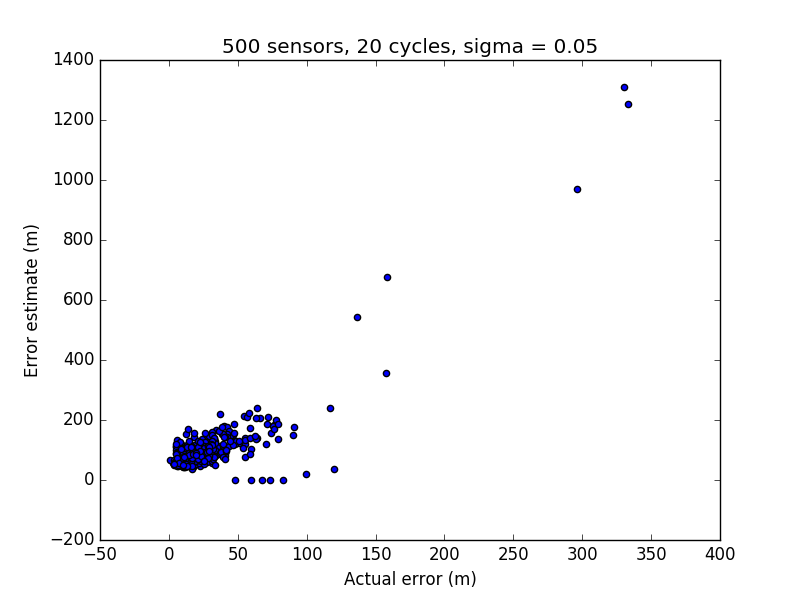
\includegraphics[scale=0.4]{img/variance2_05}
	\caption{%
	Results of post-averaging 20 samples on 500 nodes \\
	Speed of sound: 1500 ± 75 m/s \\
	Note the very wrong results caused by extreme outliers, right.
	}
\end{figure}

Unfortunately, this methods gives rather poor results. Individual samples, in conditions of high measurement errors, give very bad position estimates, and sometimes are completely wrong (by kilometres). As a result, the averaged position estimate is often quite far from the actual position, especially in cases with extreme outliers. This problem can be mitigated by eliminating the most blatant outliers, but cannot be totally eliminated.

The second method was essentially the opposite: first calculate averages and standard deviations, then calculate the position estimate. Standard deviation can be propagated through calculation in order to obtain an error estimate for the result; the Python module $unumpy$ was used to this end. This method can be called "pre-averaging". It gives better position estimates than the previous one, by roughly a factor two (not counting the outliers in the first method). However, there is little correlation between error estimates and actual localisation errors.

\begin{figure}[h]
	\centering
	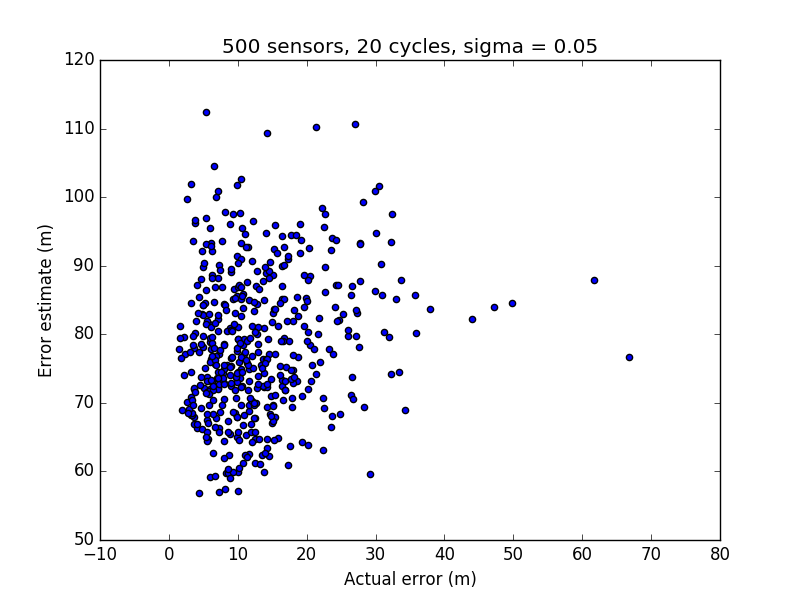
\includegraphics[scale=0.4]{img/variance1_05}
	\caption{%
	Results of pre-averaging 20 samples on 500 nodes \\
	Speed of sound: 1500 ± 75 m/s
	}
\end{figure}

The above estimation methods were empirical research; a more rigorous analysis of the localisation problem might lead to better error estimates. However, in the absence of satisfactory error estimation, the problem was mostly ignored in the implementation and testing of the following localisation schemes.

\section{LSLS tests}

\subsection{Implementation}

\begin{figure}[h]
	\centering
	\includegraphics[scale=0.25]{img/lsls-060}
	\caption{%
	LSLS in progress \\
	Yellow: localised nodes —
	Red: current anchors \\
	Blue: newly localised nodes —
	Black: unlocalised nodes
	}
\end{figure}

Unlike UPS before, LSLS was tested using a single, all-purpose class of node, since localised nodes can in turn be used as anchors. The details of the implementation (node states and message syntaxes) are described in appendix \ref{appendix:lsls}.

The anchor selection algorithm described in the article \cite{lsls} was expanded upon. Firstly, it was extended to select four anchors instead of three, since depth projection is not used here. Moreover, the algorithm as described does not offer any mechanism to handle concurrent anchor selections. If the timer of two candidates happen to finish simultaneously, or close enough that each receives the other's message after its own timer runs out, then both will think they are the legitimate anchor.

To prevent this problem, a confirmation period was added after the end of the timer. If the situation described above arises, then each of the concurrent candidates will receive the other's message during this confirmation period. They will then determine which of the two is the best fit, while the other will become candidate for the next anchor role (as if it had received the message before the end of its timer).

Because of this anchor selection process was already deemed complex enough, no provisions were made to handle transmission losses. As a result, all simulations of this method were made with no transmission loss.

Another change was the timer durations. In the article, the durations were expressed as a function of the distance to the previous anchor, but the function was ill-defined. The function used here favours anchors at intermediate range: an anchor set that is too large would not have enough overlap and would fail to locate new nodes, while one that is too small would be more prone to inaccurate localisation.

An additional restriction was put on the anchor selection algorithm: nodes can be candidate for top-level (master) anchor only once, when they have just been located. All nodes can be candidate for subsequent anchors. This has two effects: first, new anchor sets tend to be created at the edge of the localised portion of the network, where they are more likely to reach yet unlocalised nodes. Second, this provides a halting condition: once there are no more nodes to locate, the localisation process stops.

\subsection{Findings}

\begin{figure}[h]
	\centering
	\includegraphics[scale=0.25]{img/lsls-320}
	\caption{%
	Finished LSLS \\
	Yellow: localised nodes —
	Black: unlocalised nodes \\
	Note the catastrophic error build-up on the right
	}
\end{figure}

Simulations of LSLS revealed several critical issues. Some of those can be attributed to the specifics of the implementation, others are inherent to the scheme as described and would need extensive modifications to overcome.

First of all, these tests show that UPS is especially sensitive to errors in the positions of the anchors. Since LSLS is based on iterative applications of UPS, these localisation errors build up, eventually to the point where nodes become unusable as anchors because their estimated and actual positions are irreconcilable.

This is exacerbated by the fact that the anchor selection process does not account for the relative position of the anchors. As noted before, the accuracy of UPS depends in part on the judicious choice of the anchors. The distributed anchor selection algorithm has no safeguard against the creation of sub-optimal anchor sets, and modifying it to take this issue in consideration would be a complex problem.

Finally, LSLS has a tendency to stop before the entire network is localised. This flaw is caused by a specificity of the implementation: the reliance on newly localised nodes to start the anchor selection process, explained above. If an anchor set fails to localise any new node – either because of error build-up, or simply bad luck – then the localisation process stops on that front. As a result, a network above a certain size (dependent on the density) is unlikely to ever be localised entirely.

All these issues point at flaws in principles of LSLS. In particular, the distributed anchor selection algorithm does not perform its role adequately. As a consequence, rather than try to fix LSLS, a different approach was preferred.


\section{A novel method: RLS}

\subsection{Principle and implementation}

The "Request-based Localisation Scheme" (RLS) is an original localisation method. It combines the general idea of LSLS – localising an arbitrarily large network by iterative applications of UPS – and one innovation of E-UPS – letting unlocalised nodes request the anchor sets they determine to be the best.

After being initiated by the starting anchors, the localisation process consists of three repeated phases:
\begin{itemize}
	\itemsep0em
	\item An unlocalised node chose the best anchor set among its known neighbours, and broadcasts a message requesting these nodes to act as anchors.
	\item The anchors follow the usual UPS procedure, and the nearby nodes attempt to calculate a position estimate.
	\item The newly localised nodes broadcast their position to their neighbours.
\end{itemize}
Because the process is driven by the nodes that are not yet localised, it naturally ends when the entire network is localised. The stalling behaviour observed in LSLS is not possible. However, this makes the method vulnerable to transmission losses, and it was only tested without it.

In order to ensure that no concurrent requests are made, and that position broadcasts do not overlap, each node is assigned a timeslot during which it can broadcast. This assumes that the nodes' clock drift remains within known bounds for the duration of the localisation process, so that a rough synchronization is possible: not enough for precise measurements, but sufficient to avoid simultaneous transmissions. Because the duration between a node's timeslots depends on the total number of timeslots, the number of nodes in the network (or at least an upper bound) must be known in advance and inputted into each node, along with its assigned timeslot, before they are deployed. This method is particularly time-consuming, and increasingly so in larger networks, but ensures no conflicts occur. In very wide networks, this can be mitigated by assigning the same timeslots to several nodes, as long as their transmission ranges do not overlap.

Because all newly localised nodes broadcast their position, unlocalised nodes can maintain a list of anchor candidates among which they select the best anchor sets. Anchor sets are rated by several criteria, in particular their shape – sets that are closer to being coplanar receive lower ratings, and their size – like with LSLS, anchor sets should not be too large or too small. Additionally, anchors that are likely to be more accurately located are given priority, as detailed below.

\subsection{First version and findings}

\begin{figure}[h]
	\centering
	\includegraphics[scale=0.25]{img/rls-old}
	\caption{%
	Finished RLS, first version \\
	Cyan: localised nodes —
	Black: unlocalised nodes \\
	Nodes in the centre are well-localised, but in the periphery we observe error build-up
	}
\end{figure}

In a first version, each localised node was assigned an accuracy indicator, which is the number of steps between the initial anchors (assumed to be perfectly located) and the node. The initial anchors are rated 0, then the subsequent "generations" of nodes are rated 1, then 2, etc. These ratings were factored in the choice of anchor sets, under the assumption that nodes with a lower rating had more accurate position estimates.

However, simulations show that this is not sufficient to avoid the same error build-up problem that was revealed by LSLS. Position errors eventually become so great that the remaining unlocalised node are not able to calculate a position estimate, no matter what anchor set they request.

\FloatBarrier

\subsection{ToA hybrid and findings}

\begin{figure}[h]
	\centering
	\includegraphics[scale=0.25]{img/rls-new}
	\caption{%
	Finished RLS, hybrid version \\
	Cyan: ToA-localised nodes —
	Blue: UPS-localised nodes
	}
\end{figure}

Since it is apparent that UPS cannot be iterated over large networks, a hybrid UPS-ToA design was suggested. ToA was expected to be less sensitive to anchor position errors, and as a result could safely be iterated. However, only anchors would be localised by ToA: the rest of the nodes would still use UPS. Thus, this design would combine the higher accuracy and stability of ToA, with the ability of UPS to localise many nodes with comparatively few broadcasts.

The hybrid RLS design still follows the principles described above, but with one additional rule: if a UPS-localised node is requested as anchor, it must first use ToA to more accurately localise itself. To do so, it broadcasts a request, and all ToA-localised nodes nearby send a reply: the node then uses the delay between sending the request and receiving the replies to calculate a more accurate position estimate. This calculation is detailed in appendix \ref{appendix:toa}.

When choosing anchor sets, ToA-localised nodes are given priority. This is to avoid having to use ToA for an excessive number of nodes. The details of the implementation are described in appendix \ref{appendix:rls}.

As expected, simulation show the hybrid scheme is able to locate an entire network with high accuracy, and does not exhibit the error build-up problem. However, it reveals that much more nodes end up being ToA-located than expected, even with the anchor selection favouring nodes that are already ToA-located.

Moreover, analysis of the transmissions between node reveal a much heavier traffic than anticipated. In a 4x4 km network of 10x10 nodes plus 4 initial anchors, we find:

\begin{table}[H]
\centering
\begin{tabular}{|c|r|r|}
	\hline
	\multirow{4}{*}{UPS}
	& position			& 100	\\
	& requests			& 110	\\
	& beacons			& 732	\\
	& \textbf{total}	& \textbf{942}	\\
	\hline
	\multirow{4}{*}{ToA}
	& position			& 71	\\
	& requests			& 71	\\
	& replies			& 537	\\
	& \textbf{total}	& \textbf{679}	\\
	\hline
	\multicolumn{2}{|r|}{\textbf{total}}
						& \textbf{1621}	\\
	\hline
\end{tabular}
\end{table}

We see that most nodes end up broadcasting their position twice: first when they are localised by UPS, then when they are localised by ToA. Given that these messages contain the most data (three coordinates with a sufficient precision), this is a waste of bandwidth and energy. Additionally, the average number of nodes located by each request is very low.

This is possibly a consequence of a low node density. Indeed, simulating a denser network (same spatial coverage, 20x20 nodes plus 4 initial anchors) gives the following results:

\begin{table}[H]
\centering
\begin{tabular}{|c|r|r|}
	\hline
	\multirow{4}{*}{UPS}
	& position			& 396	\\
	& requests			& 175	\\
	& beacons			& 1366	\\
	& \textbf{total}	& \textbf{1937}	\\
	\hline
	\multirow{4}{*}{ToA}
	& position			& 115	\\
	& requests			& 115	\\
	& replies			& 1272	\\
	& \textbf{total}	& \textbf{1502}	\\
	\hline
	\multicolumn{2}{|r|}{\textbf{total}}
						& \textbf{3439}	\\
	\hline
\end{tabular}
\end{table}

Increasing the node density four times reduced the proportion of ToA-located nodes from 71\% to 29\%, and improved the number of UPS-located nodes per request from 0.91 to 2.26.

\chapter{Findings and analysis}

\section{UPS for small-scale localisation}

The "Underwater Positioning Scheme" possesses several qualities that make it ideal for localisation of small networks.

Since it is based on time differences, it does not require any time synchronization, either between each anchors, or between the anchors and the nodes to be localised.

It require no action on the part of the nodes to be localised: their role is entirely passive. Only the anchor send out messages. Moreover, it is distributed: each node knows its own position without a need for additional transmissions. As a result, it can be used on a network of any density, with no difference in communication overhead.

In the right conditions, it offers a good localisation accuracy. Variation of the speed of sound and transmission failures can be mitigated by repeating the process several times, in order to obtain several samples of data. However, this presumes that the anchors are well-distributed, and that their position is known with high accuracy.

\section{UPS for large-scale localisation}

Iterating UPS over a larger network is, in theory, a promising proposition. However, the simulation of two different scheme has shown that it negates much of UPS's qualities.

UPS is especially sensitive to errors in the localisation of the anchors. While this is not a problem for a one-time localisation, more than a few iterations causes the errors to add up and leads to completely erroneous position estimates. In contrast, ToA suffers from little error build-up, as demonstrated by the hybrid RLS simulations.

Likewise, the reliance of UPS on good anchor distributions suffers in iterative processes, where new anchors must be chosen out of a limited pool of candidates, with no guarantee of quality.

While the first few iterations can be expected to localise many nodes at a time, the progression at the edge of the localised portion of the network quickly becomes much slower. Eventually each iteration of UPS only localises only a few nodes, or only one, or even none. The communication overhead of UPS is relatively important, and cannot compete with ToA when it only locates nodes one at a time. Less dense networks suffer from this problem more.

\section{Prospects}

Time-of-arrival localisation had been discounted early in the project in favour of UPS, because of its high communication overhead per node localised. However, we have observed that large-scale applications of UPS suffer from this problem just as much, if not more. Moreover, the simulations of hybrid RLS show that ToA does not suffer from the same error build-up problem as UPS.

Moreover, because ToA can make use of any number of anchors at once, it is inherently resilient to transmission failure. As long as a minimum number of replies reach the node back, it will be able to calculate its position.

Therefore, it appears that ToA is a much better candidate than UPS for large-scale, iterative localisation schemes, especially in low-density networks. The groundwork for a ToA-based localisation scheme has already been laid down in hybrid RLS, and it appears that removing UPS entirely from this method could be an improvement, at least in low-density networks.

\begin{table}[H]
\centering
\begin{tabular}{|l|c|c|}
	\hline
	Hybrid RLS simulations & \textbf{6.25 nodes/km\textsuperscript{2}} & \textbf{25 nodes/km\textsuperscript{2}} \\
	\hline
	Total transmissions	& 1621			& 3439			\\
	Localised nodes		& 100			& 396			\\
	Ratio				& \textbf{16.2}	& \textbf{8.7}	\\
	\hline
	ToA transmissions	& 679			& 1502			\\
	ToA-localised nodes	& 71			& 115			\\
	Ratio				& \textbf{9.6}	& \textbf{13.1}	\\
	\hline
\end{tabular}
\end{table}

Whereas UPS has a lower communication overhead per node in higher-density networks, because more nodes can be localised at once, ToA as implemented here as a higher communication overhead per node in higher-density networks, because more nodes will answer to each localisation request. This could be mitigated by imposing restrictions on when requests are answered, so that each request is answered by a sufficient but not excessive number of nodes.

It is also conceivable to let unlocalised nodes localise themselves using passive TDoA, by listening in on other nodes' ToA localisation. This would result in a hybrid localisation method, which would improve the transmissions per localisation ratio in higher-density networks, but unlike hybrid RLS would not dedicate transmissions to TDoA localisation, resulting in a better overall communication overhead. Whether accurate TDoA localisation is possible simply by listening to ToA transmissions remains to be determined, however.

Another challenge posed by ToA localisation is the avoidance of transmissions overlap. The current call-and-reply implementation leads to many messages being received in a short time: unless messages are kept very short, collisions are bound to happen. This would need to be addressed if a ToA-based method is to be the chosen solution.

\begin{appendices}

\etocdepthtag.toc{mtappendix}
\etocsettagdepth{mtchapter}{none}
\etocsettagdepth{mtappendix}{subsection}
\etoctocstyle{1}{Appendices}
\tableofcontents‎‎

\chapter{LSLS implementation details}
\label{appendix:lsls}

\section*{Node states}

\subsection*{UNLOCALIZED}

\begin{tabular}{p{5cm}l}
	\multicolumn{2}{l}{\textbf{default starting state}} \\
	"anchor" message	& register the new anchor \\
	"beacon" message	& forget registered anchor \\
	found a complete anchor set	& become LISTENING
\end{tabular}

\subsection*{LISTENING}

\begin{tabular}{p{5cm}l}
	"beacon" message	& register data, if final beacon try to calculate position \\
	calculation successful	& become CANDIDATE \\
	calculation failed		& become UNLOCALIZED
\end{tabular}

\subsection*{LOCALIZED}

\begin{tabular}{p{5cm}l}
	\multicolumn{2}{l}{\textbf{starting state of initial anchors}} \\
	"anchor" message	& may become CANDIDATE depending on data \\
\end{tabular}

\subsection*{CANDIDATE}

\begin{tabular}{p{5cm}l}
	on state change		& set timer \\
	timer runs out		& become CONFIRMING \\
	"confirm" message	& may become LOCALIZED depending on data  \\
	"anchor" message	& may become LOCALIZED or CANDIDATE depending on data \\
\end{tabular}

\subsection*{CONFIRMING}

\begin{tabular}{p{5cm}l}
	on state change		& send "confirm", set timer \\
	timer runs out		& become ANCHOR \\
	"confirm" message	& may become LOCALIZED depending on data  \\
\end{tabular}

\subsection*{ANCHOR}

\begin{tabular}{p{5cm}l}
	on state change		& send "anchor", set a timer \\
	timer runs out		& if level 0, send "beacon" \\
	"beacon" message	& if from parent, send "beacon" \\
	last beacon			& become LOCALIZED
\end{tabular}

\section*{Messages reference}

All messages follow the format: \textbf{sender subject data} where:
\begin{itemize}
	\itemsep0em
	\item \textbf{sender} is a string that identifies the node that sent the message.
	\item \textbf{subject} is a string that indicates the purpose of the message.
	\item \textbf{data} is zero, one or more values of various types. The number of types of these values depend on the subject.
\end{itemize}

\subsection*{subject = "confirm"}

Serves to resolve conflicts between anchor candidates.

\begin{tabular}{|p{2cm}|p{2cm}|p{10cm}|}
	\hline
	\textbf{value} & \textbf{type} & \textbf{explanation} \\
	\hline
	level	& int (0-3)	&
	position in the anchor order for which the node is candidate \\
	\hline
	rating	& float		&
	number calculated from the distance to the previous anchor, indicating fitness for the anchor role \\
	\hline
	parent	& string	&
	identifier of the preceding node in the anchor order, empty if level=0 \\
	\hline
\end{tabular}

\subsection*{subject = "anchor"}

Serves to notify neighbouring nodes of the selection of a new anchor.

\begin{tabular}{|p{2cm}|p{2cm}|p{10cm}|}
	\hline
	\textbf{value} & \textbf{type} & \textbf{explanation} \\
	\hline
	level	& int (0-3)	&
	position in the anchor order \\
	\hline
	x		& float		&
	horizontal coordinate of the node \\
	\hline
	y		& float		&
	horizontal coordinate of the node \\
	\hline
	z		& float		&
	vertical coordinate of the node \\
	\hline
	parent	& string	&
	identifier of the preceding node in the anchor order, empty if level=0 \\
	\hline
\end{tabular}

\subsection*{subject = "beacon"}

Serves to localise neighbouring nodes using the UPS method.

\begin{tabular}{|p{2cm}|p{2cm}|p{10cm}|}
	\hline
	\textbf{value} & \textbf{type} & \textbf{explanation} \\
	\hline
	count	& int		&
	identifies the current broadcasting cycle \\
	\hline
	level	& int (0-3)	&
	position in the anchor order \\
	\hline
	delay	& float		&
	duration between the sending of the level 0 beacon, and the transmission of this message \\
	\hline
\end{tabular}

\chapter{RLS implementation details}
\label{appendix:rls}

\section*{Node states}

Nodes have a primary and a secondary state. There are three primary states:
\begin{itemize}
	\itemsep0em
	\item UNLOCALIZED: unlocalised node
	\item LOCALIZED: node localised by UPS, eligible to be requested as anchor
	\item ANCHOR: node localised by ToA, able to serve as anchor
\end{itemize}

\subsection*{UNLOCALIZED/idle}

\begin{tabular}{p{5cm}p{10cm}}
	\multicolumn{2}{l}{\textbf{default starting state}} \\
	on timeslot			& if anchor set found: become /requesting \\
	"position" message	& find new anchor sets \\
	"anchor" message	& modify anchor sets ratings \\
	"beacon" message	& register data, , if final beacon try to calculate position \\
	calculation successful	& become LOCALIZED/new \\
\end{tabular}

\subsection*{UNLOCALIZED/requesting}

\begin{tabular}{p{5cm}p{10cm}}
	on timeslot			& send "request" \\
	"position" message	& find new anchor sets, become /idle \\
	"anchor" message	& modify anchor sets ratings, become /idle \\
	"beacon" message	& register data, , if final beacon try to calculate position \\
	calculation successful	& become LOCALIZED/new \\
\end{tabular}

\subsection*{LOCALIZED/new}

\begin{tabular}{p{5cm}p{10cm}}
	on timeslot			& send "position", become /ready \\
\end{tabular}

\subsection*{LOCALIZED/ready}

\begin{tabular}{p{5cm}p{10cm}}
	"request" message	& if concerned, become /confirming \\
\end{tabular}

\subsection*{LOCALIZED/confirming}

\begin{tabular}{p{5cm}p{10cm}}
	on state change		& set timer \\
	timer runs out		& become /ready \\
	"ping" message		& reset timer \\
	all subsequent anchors have ANCHOR status & become /toa
\end{tabular}

\subsection*{LOCALIZED/toa}

\begin{tabular}{p{5cm}p{10cm}}
	on state change		& send "ping", set timer \\
	timer runs out		& try to calculate position \\
	"ack" message		& if concerned, register data \\
	calculation successful	& become ANCHOR/active \\
	calculation failed		& become /ready
\end{tabular}

\subsection*{ANCHOR/confirming}

\begin{tabular}{p{5cm}p{10cm}}
	on state change		& set timer \\
	timer runs out		& become /ready \\
	"ping" message		& reset timer \\
	all subsequent anchors have ANCHOR status & become /active
\end{tabular}

\subsection*{ANCHOR/active}

\begin{tabular}{p{5cm}p{10cm}}
	on state change		& if first anchor, send "beacon" \\
	"beacon" message	& if concerned, send beacon, if final beacon, become /ready \\
	all subsequent anchors have ANCHOR status & become /active
\end{tabular}

\subsection*{ANCHOR/ready}

\begin{tabular}{p{5cm}p{10cm}}
	"request" message	& if concerned, become /confirming \\
\end{tabular}

\section*{Messages reference}

All messages follow the format: \textbf{sender subject data} where:
\begin{itemize}
	\itemsep0em
	\item \textbf{sender} is a string that identifies the node that sent the message.
	\item \textbf{subject} is a string that indicates the purpose of the message.
	\item \textbf{data} is zero, one or more values of various types. The number of types of these values depend on the subject.
\end{itemize}

\subsection*{subject = "position"}

Position broadcast from a newly UPS-localised node.

\begin{tabular}{|p{2cm}|p{2cm}|p{10cm}|}
	\hline
	\textbf{value} & \textbf{type} & \textbf{explanation} \\
	\hline
	x		& float		&
	horizontal coordinate of the node \\
	\hline
	y		& float		&
	horizontal coordinate of the node \\
	\hline
	z		& float		&
	vertical coordinate of the node \\
	\hline
\end{tabular}

\subsection*{subject = "request"}

Anchor set request from an unlocalised node.

\begin{tabular}{|p{2cm}|p{2cm}|p{10cm}|}
	\hline
	\textbf{value} & \textbf{type} & \textbf{explanation} \\
	\hline
	node-0		& string		&
	first requested anchor \\
	\hline
	node-1		& string		&
	second requested anchor \\
	\hline
	node-2		& string		&
	third requested anchor \\
	\hline
	node-3		& string		&
	fourth requested anchor \\
	\hline
\end{tabular}

\subsection*{subject = "ping"}

Request of ToA localisation. No data.

\subsection*{subject = "ack"}

Reply to a ToA ping.

\begin{tabular}{|p{2cm}|p{2cm}|p{10cm}|}
	\hline
	\textbf{value} & \textbf{type} & \textbf{explanation} \\
	\hline
	node		& string		&
	node the reply is addressed to \\
	\hline
	delay		& float		&
	duration between receiving the "ping" and sending the reply \\
	\hline
\end{tabular}

\subsection*{subject = "anchor"}

Position broadcast from a newly UPS-localised node.

\begin{tabular}{|p{2cm}|p{2cm}|p{10cm}|}
	\hline
	\textbf{value} & \textbf{type} & \textbf{explanation} \\
	\hline
	x		& float		&
	horizontal coordinate of the node \\
	\hline
	y		& float		&
	horizontal coordinate of the node \\
	\hline
	z		& float		&
	vertical coordinate of the node \\
	\hline
\end{tabular}

\subsection*{subject = "beacon"}

Serves to localise neighbouring nodes using the UPS method.

\begin{tabular}{|p{2cm}|p{2cm}|p{10cm}|}
	\hline
	\textbf{value} & \textbf{type} & \textbf{explanation} \\
	\hline
	level	& int (0-3)	&
	position in the anchor order \\
	\hline
	count	& int		&
	identifies the successive broadcasting cycles \\
	\hline
	delay	& float		&
	duration between the sending of the level 0 beacon, and the transmission of this message \\
	\hline
\end{tabular}

\chapter{UPS position calculation}
\label{appendix:tdoa}

{\parindent0pt %

Consider 4 anchors $A_0$, $A_1$, $A_2$ and $A_3$, and $\mathbf{A_i} = \bigl( \begin{smallmatrix} x_i \\ y_i \\ z_i \end{smallmatrix} \bigr)$ $(0 \leq i \leq 3)$ their respective coordinates.

Let $X$ be an unlocalised node, and $\mathbf{X} = \bigl( \begin{smallmatrix} x \\ y \\ z \end{smallmatrix} \bigr)$ its coordinates.

Let $d_i$ be the distance between the node $X$ and each anchor $A_i$ $(0 \leq i \leq 3)$.

Let $\Delta_{di} = d_0 - d_i$ $(1 \leq i \leq 3)$.

\medskip

The coordinates $\mathbf{A_0}$, $\mathbf{A_1}$, $\mathbf{A_2}$, $\mathbf{A_3}$ of the 4 anchors, and the distance differences $\Delta_{d1}, \Delta_{d2}, \Delta_{d3}$ (calculated from the time differences of arrival) are the input from which the coordinates $\mathbf{X}$ of the node $X$ will be calculated.

\medskip

We have:
\begin{align}
	& d_0^2 = (\mathbf{X} - \mathbf{A_0})^2 \nonumber \\
	& d_0^2 = \mathbf{X}^2 - 2 \mathbf{A_0} \cdot \mathbf{X} + \mathbf{A_0}^2 \nonumber \\
	& \mathbf{X}^2 - d_0^2 - 2 \mathbf{A_0} \cdot \mathbf{X} + \mathbf{A_0}^2 = 0
	\label{eq:base0}
\end{align}

And, for $1 \leq i \leq 3$:
\begin{align}
	& (d_0 - \Delta_{di})^2 = d_i^2 = (\mathbf{X} - \mathbf{A_i})^2 \nonumber \\
	& d_0^2 - 2 \Delta_{di} d_0 + \Delta_{di}^2 = \mathbf{X}^2 - 2 \mathbf{A_i} \cdot \mathbf{X} + \mathbf{A_i}^2 \nonumber \\
	& \mathbf{X}^2 - d_0^2 - 2 \mathbf{A_i} \cdot \mathbf{X} + 2 \Delta_{di} d_0 + \mathbf{A_i}^2 - \Delta_{di}^2 = 0
	\label{eq:basei}
\end{align}

By subtracting \eqref{eq:base0} from each equation \eqref{eq:basei}, we obtain, for $1 \leq i \leq 3$:
\begin{align}
	& 2 (\mathbf{A_0} - \mathbf{A_i}) \cdot \mathbf{X} + 2 \Delta_{di} d_0 + \mathbf{A_i}^2 - \Delta_{di}^2 - \mathbf{A_0}^2 = 0 \label{eq:basediff}
\end{align}

This system of linear equations can be expressed in matrix form:
\begin{align}
	& \mathbf{M} \cdot \mathbf{X} + \mathbf{C} d_0 + \mathbf{D} = 0 \label{eq:main}
\end{align}

Where:
\begin{align*}
	\mathbf{M} = &
	\begin{pmatrix}
		2 (x_0 - x_1) & 2 (y_0 - y_1) & 2 (z_0 - z_1) \\
		2 (x_0 - x_2) & 2 (y_0 - y_2) & 2 (z_0 - z_2) \\
		2 (x_0 - x_3) & 2 (y_0 - y_3) & 2 (z_0 - z_3)
	\end{pmatrix} \\
	\mathbf{C} = &
	\begin{pmatrix}
		2 \Delta_{d1} \\ 2 \Delta_{d2} \\ 2 \Delta_{d3}
	\end{pmatrix} \\
	\mathbf{D} = &
	\begin{pmatrix}
		x_1^2 + y_1^2 + z_1^2 - \Delta_{d1}^2 - x_0^2 - y_0^2 - z_0^2 \\
		x_2^2 + y_2^2 + z_2^2 - \Delta_{d2}^2 - x_0^2 - y_0^2 - z_0^2 \\
		x_3^2 + y_3^2 + z_3^2 - \Delta_{d3}^2 - x_0^2 - y_0^2 - z_0^2
	\end{pmatrix}
\end{align*}

Let $\mathbf{A}$, $\mathbf{B}$ be vectors such that:
\begin{align}
	\begin{split}
		& \mathbf{M} \cdot \mathbf{A} + \mathbf{C} = 0 \\
		& \mathbf{M} \cdot \mathbf{B} + \mathbf{D} = 0
	\end{split} \label{eq:2lin}
\end{align}

Let $\mathbf{X'} = \mathbf{X} - \mathbf{B}$, then:
\begin{align*}
	& \mathbf{M} \cdot (\mathbf{X'} + \mathbf{B}) + \mathbf{C} d_0 + \mathbf{D} = 0 \nonumber \\
	& \mathbf{M} \cdot \mathbf{X'} + \mathbf{M} \cdot \mathbf{B} + \mathbf{C} d_0 + \mathbf{D} = 0 \nonumber \\
	& \mathbf{M} \cdot \mathbf{X'} + \mathbf{C} d_0 = 0 \nonumber \\
	& \mathbf{X'} = \mathbf{A} d_0
\end{align*}

Thus:
\begin{align}
	& \mathbf{X} = \mathbf{A} d_0 + \mathbf{B} \label{eq:aff}
\end{align}

From \eqref{eq:base0} and \eqref{eq:aff}, we obtain:
\begin{align}
	& (\mathbf{A} d_0 + \mathbf{B})^2 - d_0^2 - 2 \mathbf{A_0} \cdot (\mathbf{A} d_0 + \mathbf{B}) + \mathbf{A_0}^2 & = 0 \nonumber \\
	& \mathbf{A}^2 d_0^2 + 2 \mathbf{A} \cdot \mathbf{B} d_0 + \mathbf{B}^2 - d_0^2 - 2 \mathbf{A_0} \cdot \mathbf{A} d_0 - 2 \mathbf{A_0} \cdot \mathbf{B} + \mathbf{A_0}^2 & = 0 \nonumber \\
	& (\mathbf{A}^2 - 1) d_0^2 + 2 \mathbf{A} \cdot (\mathbf{B} - \mathbf{A_0}) d_0 + (\mathbf{B}^2 + \mathbf{A_0}^2) & = 0 \label{eq:quad}
\end{align}

Thus, the position of the node $X$ is found by following these steps:
\begin{enumerate}
	\item Solve the equations \eqref{eq:2lin} to obtain the vectors $\mathbf{A}$ and $\mathbf{B}$.
	\item Solve the quadratic equation \eqref{eq:quad} to obtain the distance $d_0$.
	\item If one positive solution exists, use the equation \eqref{eq:aff} to obtain the coordinates $\mathbf{X}$ of the node $X$.
\end{enumerate}
If the equation \eqref{eq:quad} has two positive solutions, a sanity check can be used to eliminate one of the two results: for example, if one of them is further away from the anchors than the communication range would allow, then it must be wrong.

}

\chapter{TOA position calculation}
\label{appendix:toa}

{\parindent0pt %

Consider $N$ anchors $A_i$, and $\mathbf{A_i} = \bigl( \begin{smallmatrix} x_i \\ y_i \\ z_i \end{smallmatrix} \bigr)$ $(1 \leq i \leq N, N \geq 3)$ their respective coordinates.

Let $X$ be an unlocalised node, and $\mathbf{X} = \bigl( \begin{smallmatrix} x \\ y \\ z \end{smallmatrix} \bigr)$ its coordinates.

Let $d_i$ be the distance between the node $X$ and each anchor $A_i$ $(1 \leq i \leq N)$.

\medskip

The coordinates $\mathbf{A_i}$ of the anchors, and the distances  $d_i$ are the input from which the coordinates $\mathbf{X}$ of the node $X$ will be calculated. This is done by solving a least-squares problem using the Gauss-Newton method.

\medskip

Let us define, for $1 \leq i \leq N$ the estimated distance and residual functions:
\begin{align*}
	& \hat{d_i}(\mathbf{X})
	= |\mathbf{X} - \mathbf{A_i}|
	= \sqrt{(x_i - x)^2 + (y_i - y)^2 + (z_i - z)^2} \\
	& r_i(\mathbf{X}) = d_i - \hat{d_i}(\mathbf{X})
\end{align*}

We seek the coordinates $\mathbf{X}$ such that $\sum\limits_{i=1}^N r_i(\mathbf{X})^2$ is minimal. The Gauss-Newton algorithm starts with an initial guess $\mathbf{X^{(0)}}$ and refines it by the following process:

\begin{align*}
	& \mathbf{X^{(n+1)}} = \mathbf{X^{(n)}} - (\mathbf{J_r}^\top \cdot \mathbf{J_r})^{-1} \cdot \mathbf{J_r}^\top \cdot \mathbf{r}(\mathbf{X^{(n)}})
\end{align*}

Where $\mathbf{r}(\mathbf{X}) = \bigg( \begin{smallmatrix} r_1(\mathbf{X}) \\ \vdots \\ r_N(\mathbf{X}) \end{smallmatrix} \bigg)$ is the vector of residuals and $\mathbf{J_r}$ is its Jacobian matrix.

\medskip

For $1 \leq i \leq N$, we have:
\begin{align*}
	& (\mathbf{J_r})_{i,1}
	= \frac{\partial r_i}{\partial x}(\mathbf{X})
	= - \frac{\partial d_i}{\partial x}(\mathbf{X})
	= \frac{(x_i - x)}{\sqrt{(x_i - x)^2 + (y_i - y)^2 + (z_i - z)^2}}
	= \frac{(x_i - x)}{d_i(\mathbf{X})} \\
	& (\mathbf{J_r})_{i,2}
	= \frac{\partial r_i}{\partial y}(\mathbf{X})
	= \frac{(y_i - y)}{d_i(\mathbf{X})} \\
	& (\mathbf{J_r})_{i,3}
	= \frac{\partial r_i}{\partial z}(\mathbf{X})
	= \frac{(z_i - z)}{d_i(\mathbf{X})}
\end{align*}

This refining process is repeated until either the difference $\mathbf{X^{(n+1)}} - \mathbf{X^{(n)}}$ becomes lower than a set threshold, or a maximum number of iteration is reached.


\medskip

As long as there are not multiple minima (4 anchors or more), this algorithm converge quickly, even with an arbitrary initial guess. In simulations, with an initial guess $\mathbf{X^{(0)}} = \big( \begin{smallmatrix} 0 \\ 0 \\ 0 \end{smallmatrix} \big)$, a threshold of 0.01 m is almost always reached in less than 10 iterations.

}

\end{appendices}

\etocdepthtag.toc{mtchapter}

\begin{thebibliography}{10}
\addcontentsline{toc}{chapter}{Bibliography}
	\bibitem{survey}
		Q. Fengzhong, W. Shiyuan, et al.
		{\em "a survey of ranging algorithms and localization schemes in underwater sensor networks"},
		 China Communications 13.3,
		 66-81,
		 2016.
	
	\bibitem{ups}
		X. Cheng, H. Shu, et al.
		{\em “silent positioning in underwater acoustic sensor networks”},
		IEEE Transactions on Vehicular Technology 57.3,
		1756-1766,
		2008.
	
	\bibitem{eups}
		H.P Tan, Z.A. Eu, W.K.G. Seah,
		{\em “an enhanced underwater positioning system to support deepwater installations”},
		Proc. OCEANS 2009, Biloxi, MS, USA,
		1-8,
		2009.
	
	\bibitem{lsls}
		W. Cheng, A. Thaeler, et al.
		{\em “time-synchronization free localization in large scale underwater acoustic sensor networks”},
		Proc. 29th IEEE ICDCS, Montreal, Canada,
		80–87,
		2009.
	
%	\bibitem{3dul}
%		M.T Isik, O.B Akan,
%		{\em “a three-dimensional localization algorithm for underwater acoustic sensor networks”},
%		IEEE Transactions on Wireless Communications 8.9,
%		4457-4463,
%		2009.
%	
%	\bibitem{mhml}
%		A. Savvides, H. Park, M.B. Srivastava,
%		{\em "the bits and flops of the n-hop multilateration primitive for node localization problems"},
%		Proc. 1st ACM Int. workshop on Wireless sensor networks and
%applications, Atlanta, GA, USA,
%		2002.
\end{thebibliography}

\end{document}